% !TeX document-id = {c68ea1ac-ebac-4541-a297-17005c6d2297}
% !TeX encoding = UTF-8
% !TeX spellcheck = en_US
% !TeX TS-program = pdflatex
% !TeX TXS-program:bibliography = biber -l zh__pinyin --output-safechars %

\documentclass[10pt]{article}

% to be `\input` in subfolders,
% ... therefore the path should be relative to subfolders.

\usepackage{iftex}
\ifPDFTeX
\else
	\usepackage[UTF8
		,heading=false
		,scheme=plain % English Document
	]{ctex}
\fi
%\ctexset{autoindent=true}
%\usepackage{indentfirst}
\setlength{\parindent}{0pt}

\input{../.modules/basics/macros.tex}
\input{../.modules/preamble_base.tex}
%\input{../.modules/preamble_notes.tex}
\input{../.modules/basics/biblatex.tex}


%Misc
%	\usepackage{lilyglyphs}
%	\newcommand{\indicator}{$\text{\clefG}$}
%	\newcommand{\indicatorInline}{$\text{\clefGInline}$}

\usepackage{titling}

\hypersetup{%
	colorlinks=true
	,linkcolor=DarkBlue
	,urlcolor=purple
	,linktoc=all
}


% Settings
\counterwithout{equation}{section}
\mathtoolsset{showonlyrefs=false}
%\DeclareTextFontCommand{\textbf}{\sffamily}

% Spacing
\usepackage[
	papersize={32cm,40cm},
	hmargin=1.5cm,
	vmargin={1.5cm,1.7cm}
]{geometry}
\geometry{footnotesep=2\baselineskip} % pre footnote split
\setlength{\parskip}{.5\baselineskip}
\renewcommand{\baselinestretch}{1.15}

\usepackage{ragged2e}

\usepackage{multicol}
\setlength{\columnsep}{2em}
\usepackage{enumitem}


%% List
	\setlist*{
%		noitemsep,
%		listparindent=\parindent
%		,labelindent=\parindent
%		parsep=\parskip
		nosep,
		parsep=\parskip,
		leftmargin=1.5em
	}


\usepackage{tikz}
\usepackage{caption}
%\usepackage{snapshot}

\renewenvironment{frame}[1]%
	{\section*{#1}}%
	{}

\newcommand{\citations}[1]{{\footnotesize#1\par}}
\newcommand{\reality}{reality\textsuperscript{TM}}

%\subtitle{An extended AdS\,/\,\TTbar duality \textit{(beyond infinity)}}


\newcommand{\veccol}[1]{\pqty{
	\begin{smallmatrix}
		#1
	\end{smallmatrix}
}}

\addbibresource{glueon-beamer.bib}
%\usepackage{cprotect}

\usepackage{cancel}
\newcommand{\slot}{{\,\bullet}}

\usepackage{xspace}
\newcommand{\TTbar}{\texorpdfstring{\ensuremath{T\bar{T}}}{TTbar}\xspace}

\newcommand{\jokeInfinity}{
	\includegraphics[height=.2\linewidth]{img/smbc-cantor-cropped.png}
\\[-.5ex]
	{\footnotesize\url{https://smbc-comics.com/comic/cantor}}
}

\setlength{\droptitle}{-3.25\baselineskip}
\pretitle{\LARGE\bfseries\noindent}
\title{Glue-on AdS holography for $T\bar T$-deformed CFTs}
\posttitle{\ \footnotesize\textsl{JHEP 06 (2023) 117}}

\preauthor{\par\large\noindent}
\author{%
	Luis Apolo,
	Peng-Xiang Hao \textkai{\normalsize 郝鹏翔},
	\textbf{Wen-Xin Lai \textkai{\small 赖文昕}},
	and Wei Song \textkai{\small 宋伟}
}
\postauthor{
	\,\arxiv{2303.04836}
	\par%\vspace{.5\baselineskip}
	\vspace{-.6\baselineskip}
	\noindent\rule{.68\linewidth}{1pt}\par
	\vspace{-.1\baselineskip}
%	\vspace{.3\baselineskip}
}

\predate{\noindent\sffamily%
	\begin{minipage}{3em}
		\includegraphics[width=2.7em]{img/ymsc-logo.pdf}
	\end{minipage}
	Yau Mathematical Sciences Center YMSC, Tsinghua
	---
}
\date{September 2023}
\postdate{
	@ YITP, Kyoto
%	\vspace{0\baselineskip}
}

\pagestyle{empty}

\begin{document}

\maketitle
\thispagestyle{empty}


\begin{multicols}{3}

%\textbf{Abstract:}
\,\\[-2.2\baselineskip]

\TTbar-deformed CFTs with $\mu < 0$ have been proposed by \mbox{\textcite{McGough:2016lol}} to be holographically dual to Einstein gravity with a finite \mbox{Dirichlet} cutoff.

We generalize the proposal for $\mu > 0$ by \textit{gluing-on} another patch of $\mrm{AdS}_3$, and \mbox{provide} various evidence for this extended holography, now valid for $\mu \in \mbb{R}$.

\vspace{.8\baselineskip}
\hrule
\vspace{.3\baselineskip}

\textbf{Pure Einstein gravity} without matter in $\mrm{AdS}_3$:
\begin{align}
\hspace{-.8em}
	ds^2
	&= \ell^2 \bigg( \frac{d\rho^2}{4 \rho^2} + \frac{ \big( du + \rho \, \mathcal {\bar L}(v)\, dv \big) \big( dv + \rho \, \mathcal L(u)\, du \big) }{\rho} \bigg) \notag\\
	&= n_\mu n_\nu dx^\mu dx^\nu + \frac{1}{\zeta} \gamma_{ij}dx^i dx^j, \label{fggauge}
\end{align}

\begin{itemize}
\item Transverse coordinates: $x^{i} \sim \varphi, t$ \\
	Light-cone coordinates: $u,v = \varphi \pm t$

	$\mathcal L(u), \bar{\mathcal L}(v)$: arbitrary periodic functions
\item Radial coordinate: $
	\ell^{-2} g_{\varphi\varphi} \equiv r^2 \equiv \zeta^{-1}$\\
	$r$: the ``proper radius''
\end{itemize}
\begin{center}
	\vspace{-.5\baselineskip}
	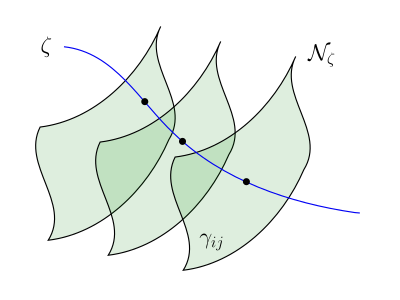
\includegraphics[width=.52\linewidth]{img/foliation.pdf}
	
	\vspace{-.3\baselineskip}\scriptsize
	Image courtesy: \textsl{R. Szalai},\\
	\tiny\texttt{DOI:10.1007/s11071-020-05891-1}

	\vspace{-.5\baselineskip}
\end{center}
\begin{itemize}
\item Structure: foliated by constant $\zeta$ surfaces ${\mathcal N}_\zeta$\\[.6ex]
Asymptotic boundary: $\mcal{N}_0$ is at $\zeta \to 0$
\\[1ex]
\citations{%
	\textcite{Fefferman:2007rka}\\
	\textcite{Banados:1992wn}%\\
%	\textcite{Banados:1998gg}
}
\end{itemize}

\textbf{``$\thinmspace[.9]\TTbar$\,'' deformation} as the flow of action:
\begin{align}
\hspace{-.1em}
	\partial_{\sidenote{\mu}} I &= {8 \pi} \int d^2x \, T\bar T_{(\sidenote{\mu})} = {\pi} \int d^2x\,\big( T^{ij}T_{ij}- (T^i_i)^2 \big)_{(\sidenote{\mu})},\notag\\
	&x, \bar{x} = \varphi' \pm t'
	\label{TTbardef}
\end{align}

\begin{itemize}

\item \textbf{Irrelevant:} initially $\mrm{CFT}_2$: $T\bar{T}_{(\mu = 0)} = T_{xx} T_{\bar{x}\bar{x}}$, \\
but conformal symmetry will be broken for $\mu \ne 0$.

\item \textbf{Solvable:} the deformed spectrum of $\hat{H}(\mu)$ and $\hat{J}(\mu)$ on a cylinder of radius $R$ is a simple function:
\begin{equation}
\hspace{-2em}
\begin{gathered}
	E(\mu) = - \frac{R }{ 2\mu } \bigg(1-\sqrt{1 + \frac{4\mu}{R} E(0) + \frac{4\mu^2}{R^4} J(0)^2 }
	\,\bigg), \\ J(\mu)=J(0) \\[-1.5ex]
\end{gathered} \label{ttbarspectrum}
\end{equation}
of the undeformed spectrum $E(0)$, $J(0)$.\\
(\textit{under reasonable assumptions})

\citations{
\textcite{Zamolodchikov:2004ce}\\
\textcite{Dubovsky:2012wk}\\
\textcite{Dubovsky:2013ira}\\
\textcite{Smirnov:2016lqw}\\
\textcite{Cavaglia:2016oda} \textit{et al}%\\
%\textcite{Dubovsky:2017cnj} 
}

\vspace{-.8\baselineskip}

\end{itemize}

\subsection*{Cutoff $\mrm{AdS}_3$ duality:\texstringonly{\\} Holography within a finite Dirichlet wall}
\vspace{-.2\baselineskip}
\citations{
\textcite{McGough:2016lol}\\
\textcite{Kraus:2018xrn} \textit{et al}
}

\textbf{Dictionary:} radial location $\zeta_c$ of the cutoff surface $\mcal{N}_{\zeta_c}$ gets mapped to the deformation parameter $\mu$:
\begin{equation}
	\zeta_c = - \frac{c \mu}{3\ell^2}
	\label{dictionary}
\end{equation}
\TTbar flow recast geometrically as the $i,j$ components of the Einstein equations. 

This is a ``non-AdS'' / non-CFT duality.\\
\textit{A step towards quantum gravity in \reality!}

\textbf{Caveat:} the duality only admits $\zeta_c > 0$ so $\mu < 0$.\\
But \TTbar itself admits $\mu > 0$ with nice properties.

\citations{The related proposal of \textcite{Guica:2019nzm}\\
admits both signs of $\mu$.}

\textit{What is the other side of the duality?}

\columnbreak

\vspace*{-3.6\baselineskip}
\begin{center}
	\mbox{
		\hspace{-1.55em}
		\includegraphics[width=1.14\linewidth]{img/ads-cft-cutoff.png}
	}
	
	\vspace{-.8\baselineskip}\small
	Cutoff $\mrm{AdS}_3$\,/\,\TTbar-deformed $\mrm{CFT}_2$

	\vspace{-.3\baselineskip}
	\scriptsize\ Image courtesy: \textcite{AldegundePWSep22}
\end{center}


%\begin{itemize}
%
%\item[] \textbf{Caveat:} the duality only admits $\zeta_c > 0$ so $\mu < 0$.\\
%But \TTbar itself admits $\mu > 0$ with cool properties.
%
%\citations{The related proposal of \textcite{Guica:2019nzm}\\
%admits both signs of $\mu$.}
%
%\textit{What is the other side of the duality?}
%
%\end{itemize}

\vspace{-1.5\baselineskip}

\section*{\textbf{Proposal:}\texstringonly{\\}Glue-on $\mrm{AdS}_3$ -- beyond the infinity}
\label{se:glueonproposal}

\parbox{\linewidth}{
\vspace{-\baselineskip}
\textbf{\begin{equation*}
\hspace{-2.8em}
\begin{aligned}
	\textrm{Cutoff}
	\ &/\ %
	\text{\textit{glue-on} $\mrm{AdS}_3$ Gravity}
	\!\!&\equiv\ %
	\textrm{\TTbar deformed $\mrm{CFT}_2$ at $\mcal{N}_{\zeta_c}$} \\
	\zeta_c > 0
	\ &/\ %
	\zeta_c < 0
	& \mu \in \mbb{R}\hspace{1em}\,
\end{aligned}
\end{equation*}}
\begin{center}
	\vspace{-1\baselineskip}%

	\centering
	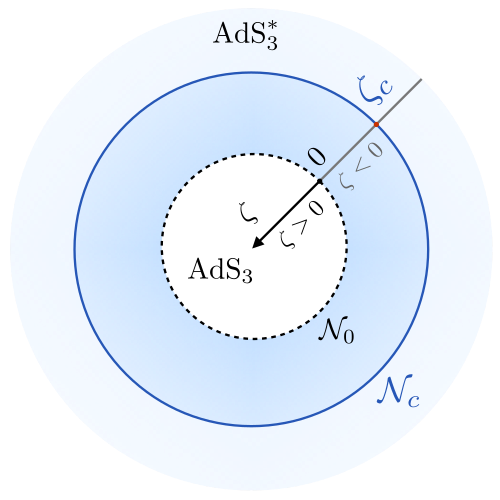
\includegraphics[width=.8\linewidth]{img/diagram.png}
	
	\scriptsize\ Top-down view of a constant $t$ slice
\end{center}
%\vspace{-\baselineskip}
}

\begin{itemize}

\item The metric \eqref{fggauge} has a simple pole, thus admits a well-defined \textbf{analytic continuation:}
%\begin{equation}
%	\rho,\ \zeta,\ \mu\ \in\ \mbb{R}
%\end{equation}
\begin{equation}
	\frac{1}{\zeta} \equiv \ell^{-2} g_{\varphi\varphi} \in \mbb{R},
\ \quad
	\zeta_c = - \frac{c \mu}{3\ell^2} \in \mbb{R}
\end{equation}
What are we doing other than copy-pasting?\\
``Renormalize'' the divergences as $\zeta \to 0^\pm$:
	\begin{itemize}[noitemsep]\small
	\item introduce $\mathcal N_{\zeta={\pm\epsilon}}$ and \textbf{``glue''} them together;
	\item i.e.~exclude the $-\epsilon < \zeta < \epsilon$ region, \\ until finally sending $\epsilon \to 0$. 
	\end{itemize}
	
\item \textbf{Extending the flow:} matching energy momentum (Brown-York) \& the \TTbar flow equations:
	\begin{equation}
	\begin{gathered}
		T_{ij}= \frac{\sigma_{\zeta_c}}{8\pi G} \Big( K_{ij} -  K \gamma_{ij} + \frac{1}{\ell |\zeta_c|}\gamma_{ij}\Big), \\ \sigma_{\zeta_c} = \tfrac{\abs{\zeta_c}}{\zeta_c} = \pm 1,\quad
		\gamma_{ij} = \zeta_c h_{ij}, \\[-1ex]
	\end{gathered}	\label{BYtensor}
	\end{equation}
	$h_{ij}$: the induced metric. 
	
	The field theory metric $\gamma_{ij}$ is always positive-definite, while $h_{ij}$ becomes negative-definite for the glue-on region $\rho,\zeta < 0$.
	
	This discrepancy is the origin of $\abs{\zeta_c}$.

%\end{itemize}
%
%\subsection*{\TTbar physics from the glue-on geometry}
%
%\begin{itemize}

\item Demanding a \textbf{non-singular extended geometry} reproduces bounds on the \TTbar deformed theory, e.g.
	\begin{equation}
		\zeta_c \ge -1 \quad \Leftrightarrow \quad\mu\le \frac{ 3\ell^2 }{c} \label{reality}
	\end{equation}
	This is a Killing horizon in the glue-on region of the \mbox{extended} geometry;
	$(\det g_{\mu\nu})_{\,\zeta = -1} = 0$.

\item \textbf{Spectrum from the extended geometry:} they are \mbox{conserved} charges $\mcal{Q}$ of the Killing symmetries, and can be computed with the \textit{covariant formalism}.

\citations{
	\textsl{\citeauthor{Iyer:1994ys,Barnich:2001jy}} et al\\
	With \TTbar: \textcite{Kraus:2021cwf}
}\vspace{-1.5\baselineskip}
	\begin{align*}
		\delta E(\mu) &\equiv  \ell^{-1} \delta \mathcal Q_{\pd_{t'}}, \quad \delta J(\mu) \equiv  \delta \mathcal Q_{\pd_{\varphi'}}.
	\end{align*}
	This reproduces $E(\mu)$, $J(\mu)$ with $\mu \in\mbb{R}$ in \eqref{ttbarspectrum}.\\
	$(t',\varphi')$: normalized boundary coordinates:
	\begin{equation}
		ds^2_c = \ell^2 ( -dt'^2 + d\varphi'^2) , \qquad \varphi' \sim \varphi' + 2\pi.\label{cutoffmetric}
	\end{equation}

\columnbreak

\vspace*{-8\baselineskip}
%\item The covariant charges (variation):

	\item \textbf{\textit{State-dependent} maps of \mbox{coordinates}:}
	\begin{align}
		dt' &= \sqrt{ \big(1 - \zeta_c (T_u+T_v)^2 \big) \big(1 - \zeta_c (T_u-T_v)^2 \big) } \, dt, \notag \\
		 d\varphi' &= d\varphi + \zeta_c \big( T_u^2 - T_v^2 \big)\,dt.
	\label{eq:state_dependent_map}
	\end{align}
	$\leadsto$ correct charges, the modified signal propagation speed $v'_{\pm} \equiv \pm {d\varphi'}/{dt'}$, and \TTbar \textbf{thermodynamics} upon Wick rotation. In particular,
	\begin{equation*}
	\hspace{-.8em} \mu > 0,\ \ \,
		T_L(\mu)\,T_R(\mu) \le - \frac{1}{4\pi^2 \ell^2 \zeta_c} = \frac{3}{4\pi^2c\mu} = T_H(\mu)^2.
	\end{equation*}
	$T_{L,R}$: temperatures associated with $u',v' = \varphi' \pm t'$.\\
	$T_H$: the \textit{Hagedorn temperature}: exceeding $T_H$ leads to a complex entropy.

\begin{flushright}
\vspace{-.5\baselineskip}
\citations{
\textcite{Giveon:2017nie}\\
\textcite{Apolo:2019zai}
}
\vspace{-.8\baselineskip}
\end{flushright}

\end{itemize}

\subsection*{\TTbar partition functions from the bulk} \label{se:partitionfunction}

\begin{itemize}
\item Via bulk on-shell action of the dominant saddle:
	\begin{equation}
		Z_{T\bar T} (\mu) = \mathcal Z (\zeta_c) \approx  e^{-I(\zeta_c)}. \label{partition2}
	\end{equation}
$I(\zeta_c)$ \mbox{diverges} at $\zeta \to 0^\pm$: we need \textit{holographic renormalization}, with the boundary action:
	\begin{align}
%		I_{\mcal{M}}(\zeta_1, \zeta_2) & \coloneqq - \frac{1}{16\pi G} \int_{\zeta_1}^{\zeta_2} d\zeta \int d^2 x \sqrt{g} \, (R + 2 \ell^{-2}),  %\label{bulkaction} \\
%	\\
		I_{\mathcal N_{\zeta}} & \coloneqq  - \frac{1}{8\pi G} \int_{\mathcal N_{\zeta}} d^2x \sqrt{h}\,h^{ij} K_{ij} \label{boundaryaction}
	\\& \qquad + \frac{\sigma_\zeta}{8\pi G} \int_{\mathcal N_{\zeta}} d^2x \sqrt{h} \, \bigg(\ell^{-1} - \frac{\ell  \mathcal{R}[h]}{4} \log |\zeta| \bigg). \notag
	\end{align}
	\hfill{\footnotesize \textcite{Henningson:1998gx} \textit{et al}}

	$\log |\zeta|$: not diff-invariant, due to the Weyl anomaly. \\
	$I_{\mcal{N}_\zeta}$: consistent with the B-Y stress tensor \eqref{BYtensor}.
	
	$Z_{\TTbar}$ agrees with the field theory analysis, using \eqref{eq:state_dependent_map}:

\item \textbf{Torus:} {modular invariance} \& sparseness of the ``light'' spectrum at large $c$ $\leadsto$ universal form:
	\begin{equation*}\small
	\hspace{-2.8em}
		\log Z_{T\bar T}(\mu)  \approx \left\{ \begin{aligned}
		& {-\frac{1}{2}}\,(\beta_L + \beta_R)\, RE_{\text{vac}}(\mu),  &\beta_L \beta_R > 1, \\
		& {-2 \pi^2 \bigg(\frac{1}{\beta_L} + \frac{1}{\beta_R}\bigg)  RE_{\text{vac}}\bigg(\frac{4\pi^2}{\beta_L \beta_R} \mu \bigg)},  &\beta_L\beta_R < 1. %\\[2ex]
		 \end{aligned} \right. %\label{ZTTbar}
	\end{equation*}
	\begin{flushright}
		\vspace{-.5\baselineskip}
		\citations{\noindent%
			\textcite{Datta:2018thy}\\
			\textcite{Apolo:2023aho}\\
			cf.~\textcite{Hartman:2014oaa}
		}
		\vspace{-.5\baselineskip}
	\end{flushright}

\item \textbf{Sphere:} maximally symmetric,\\[-1.4\baselineskip]

\hfill\mbox{\footnotesize \textcite{Donnelly:2018bef}}
	\begin{equation}
%		\label{sphere:stresstensor}
		\langle T_{ij}\rangle = -\frac{1}{4\pi\mu} \bigg(1-\sqrt{1-\frac{c\mu}{3R^2}}\, \bigg)  \gamma_{ij}.
	\end{equation}
Trace relation: \mbox{$
%	\begin{align*}
%\partial_\mu \log Z_{\TTbar}(\mu)&=8\pi \int d^2x\sqrt{\gamma}\, \langle T\bar{T} \rangle \\
(-R)\,\partial_R \log Z_{\TTbar}(\mu)=\int d^2x\sqrt{\gamma}\,\langle T^i_i \rangle
%	\end{align*}
$} and the flow equation \eqref{TTbardef} 
admit the general \mbox{solution} with a $\mu$-\textit{independent} integration constant $a$:
	\begin{equation*}\small
	\hspace{-1.8em}
		\log Z_{\TTbar}(\mu, a) = \tfrac{c}{3} \log \Big[\tfrac{R}{a}   \Big(1+\sqrt{1-\tfrac{c \mu }{3  R^2}}\, \Big) \Big] - \tfrac{R^2}{\mu}  \sqrt{1-\tfrac{c \mu }{3 R^2}} + \tfrac{R^2}{\mu}. %\label{Zsol}
	\end{equation*}
	\begin{itemize}%[noitemsep]
	\item $a = \sqrt{c|\mu|/3}$: \mbox{recover {\small
		\textsl{\citeauthor{Donnelly:2018bef}}
		\cite{Donnelly:2018bef}
	}} \\
	$a = \epsilon$: also a valid choice, where the RG length scale $\epsilon$ is decoupled from $\mu$.
	
	\item Enlarge the \textbf{space of \TTbar deformed theories:}\\
	with \mbox{independent} parameters $(\mu,a)$.
	
	\item The $\log |\zeta|$ in \eqref{boundaryaction} guarantees that $I = -\log Z_{\TTbar}$ \mbox{satisfies} the $T\bar T$ flow \eqref{TTbardef}; not the case for \cite{Donnelly:2018bef}.
	\end{itemize}

	
	\begin{flushright}
		\vspace{-.6\baselineskip}
		\citations{
			\textcite{Caputa:2020lpa}\\
			\textcite{Li:2020zjb}
		}\vspace{-.8\baselineskip}
	\end{flushright}
	
	\item Future: understand the \textbf{entanglement structure} of \TTbar deformation with the help of bulk geometry.
	\begin{flushright}
		\vspace{-.5\baselineskip}
		\citations{
			\textcite{Lewkowycz:2019xse}
		}
	\end{flushright}
\end{itemize}
\centering\vspace{-1\baselineskip}
\includegraphics[width=.6\linewidth]{img/RT-AdS.pdf}

\vspace{-1\baselineskip}
{\footnotesize RT surface for the extended $\mrm{AdS}_3$}

\vspace{.8\baselineskip}
\hrule
\vspace{.1\baselineskip}

\hspace{-.7em}
\begin{minipage}[c]{.81\linewidth}
\begin{itemize}[noitemsep,leftmargin=5em]\small
\item[\texttt{Email:}]
	\url{bryanlais@gmail.com}
\item[\texttt{Inspire:}]
	\href{https://inspirehep.net/authors/2640135}{
		\texttt{inspirehep.net/authors/2640135}
	}
\item[\texttt{GitHub:}]
	\href{https://github.com/bryango}{
		\texttt{github.com/bryango}
	}
\end{itemize}
\end{minipage}%
\hfill%
\begin{minipage}{.17\linewidth}
\includegraphics[width=\linewidth]{img/inspire-qr-cy.png}
\end{minipage}%
~\mbox{}

\end{multicols}

\end{document}
